\documentclass{article}
\usepackage{amssymb}
\usepackage{graphicx}
\usepackage{float}
\usepackage{appendix}
\usepackage[final]{corl_2025}

% fix bug in corl_2025
\makeatletter
\providecommand{\@notice}{}
\makeatother

\title{GestureBot - Intuitive Robot Arm Control via Hand Tracking}

% The \author macro works with any number of authors. There are two
% commands used to separate the names and addresses of multiple
% authors: \And and \AND.
%
% Using \And between authors leaves it to LaTeX to determine where to
% break the lines. Using \AND forces a line break at that point. So,
% if LaTeX puts 3 of 4 authors names on the first line, and the last
% on the second line, try using \AND instead of \And before the third
% author name.

% NOTE: authors will be visible only in the camera-ready and preprint versions (i.e., when using the option 'final' or 'preprint'). 
% 	For the initial submission the authors will be anonymized.

\author{
  Alexander Neary\\
  University of California Los Angeles \\
  CS 188, Yuchen Cui\\
  \And
  Brenna Kjorness\\
   University of California Los Angeles \\
  CS 188, Yuchen Cui\\
  \And
    Clayton Castro\\
     University of California Los Angeles \\
  CS 188, Yuchen Cui\\
}


\begin{document}
\maketitle{}

%===============================================================================


%===============================================================================

\section{Problem Statement}

Modern robotic manipulators often rely on complex interfaces or pre-programmed
sequences for control, making them less accessible for intuitive, real-time
human interaction. In many applications—such as assistive robotics,
teleoperation, or educational tools—natural, gesture-based control systems can
significantly enhance usability and responsiveness. However, developing a
reliable and low-latency gesture recognition system that translates human hand
movements into precise robot arm control, especially in multiple degrees of
freedom, remains a technical challenge. This project addresses the problem by
designing GestureBot, an intuitive robot arm interface controlled entirely
by hand gestures using a single RGB camera. By leveraging computer vision
techniques with OpenCV and MediaPipe, GestureBot aims to enable full 6DoF
(degrees of freedom) control—translational and rotational—of the robot’s end
effector, as well as gripper operation via pinching gestures, without any
physical input devices. The core problem tackled is the effective mapping of
human hand motion to robotic motion in real-time, enabling the robot to
complete complex manipulation tasks such as turning a door handle and stacking
blocks.

%===============================================================================

\section{System Design / Methodology}
\label{sec:citations}



\subsection{MediaPipe Hand Tracking}
MediaPipe is a machine-learning-powered library that can detect hands using a
monocular camera. MediaPipe is able to infer 21 3D landmarks of the hand, as
seen in [\citealp{MediaPipeHands}, Fig.~1]. We set up hand tracking using
MediaPipe\cite{MediaPipeGuide}, with MediaPipe doing the heavy lifting in terms
of detecting/tracking the hand and creating landmarks for each part of the
hand. After iteration and testing, we added an additional landmark that is
normal to the palm to assist rotation computation. 

\begin{figure}[H]
  \centering
  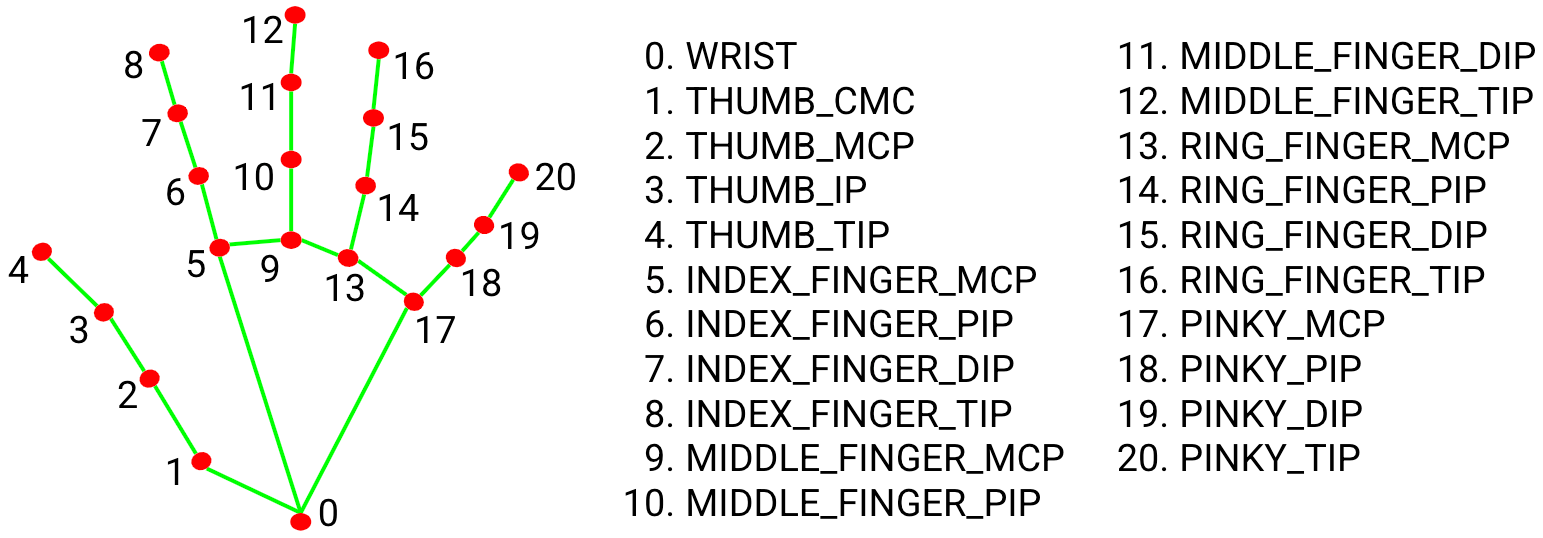
\includegraphics[width=0.7\textwidth]{../assets/hand_landmarks.png}
  \caption{21 hand landmarks tracked by MediaPipe.}
  \label{fig:hand-landmarks}
\end{figure}
\subsection{OpenCV}
Open Computer Vision was utilized to convert the camera colors and set up the
webcam. Additionally, using OpenCV we could create the visual indicators for
each of the 21 created landmarks, so we understood exactly how the hand was
being tracked (see Figure \ref{fig:hand-landmarks-webcam}).
\begin{figure}[H]
  \centering
  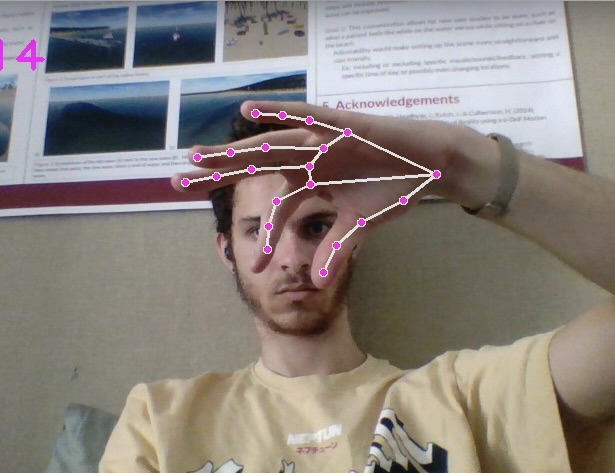
\includegraphics[width=0.7\textwidth]{../assets/hand-landmarks-webcam.jpeg}
  \caption{21 hand landmarks tracked by MediaPipe overlayed on a hand using OpenCV.}
  \label{fig:hand-landmarks-webcam}
\end{figure}
\subsection{Coordinate System Conversion}
The MediaPipe axes and coordinate systems are different from the Robosuite
system, so we had to do conversions and scaling to translate the coordinates.
Robosuite also expects the robot end-effector to start at (0,0,1), while the
Mediapipe expects (0,0,0), so we tweaked the origins. 
\subsection{Depth Calculation}
The built-in depth coordinates in MediaPipe are only relative to the wrist, so
they are better for calculating pose than depth. By using a single point (other
than the wrist, since its Z value stays constant) and extracting its depth, we
could maintain depth tracking that also allowed for hand rotation. We created
two linear relationships: one for the depth of that point when tracked in the
webcam, and the other for the depth of the end effector in the Robosuite
simulation. Then we could interpolate the depth of the end effector by using
the depth of the tracked landmark. Then we added this computed depth to the
height and width of the wrist and updated the PID with the new target, allowing
for a full range of translational motion.

\subsection{Rotation Calculation}
We created a set of axes from the hand landmarks to calculate rotation. We used
the normalized vector from the wrist to the thumb, the normalized vector from
the wrist to the pinky, and then created an orthogonal vector that points
normal to the palm. With our newly defined X, Y, and Z axes, we created a
rotation matrix and utilized scipy.spatial.transform to transform the matrix
into a rotation vector. Once computed, the rotation of the end effector
(\texttt{robot\_eef\_quat}) is evaluated and compared to the computed rotation
vector to find the change in rotation (\texttt{delta\_rot}) which can be added
to the rotation portion of the action array. Once we added isolating
translation and rotation, we adjusted the rotation calculation to be relative
to a "base rotation", computed when you first make your left hand into a fist
after it was open in the previous frame. 

\subsection{Isolating Rotation and Translation}
We were finding it difficult to control both rotation and translation of our
hand at the same time to move the robot. For example, when trying to rotate
your hand, you inadvertently move it translationally, and vice versa. We
remedied this by using the left hand to toggle between rotation and
translation. If you make your left hand into a loose fist, your right hand can
rotate the end effector, as seen in Figure \ref{fig:fist-rotation}. When your
left hand is not in a fist or is off-screen, your right hand controls the
translation of the end effector. The fist gesture is recognized by taking the
angles between the joints on your hand to detect curling of the fingers.
MediaPipe can have difficulty detecting the coordinates of your fingers when
they are fully curled, so we kept the threshold for fist detection loose. 
\begin{figure}[H]
  \centering
  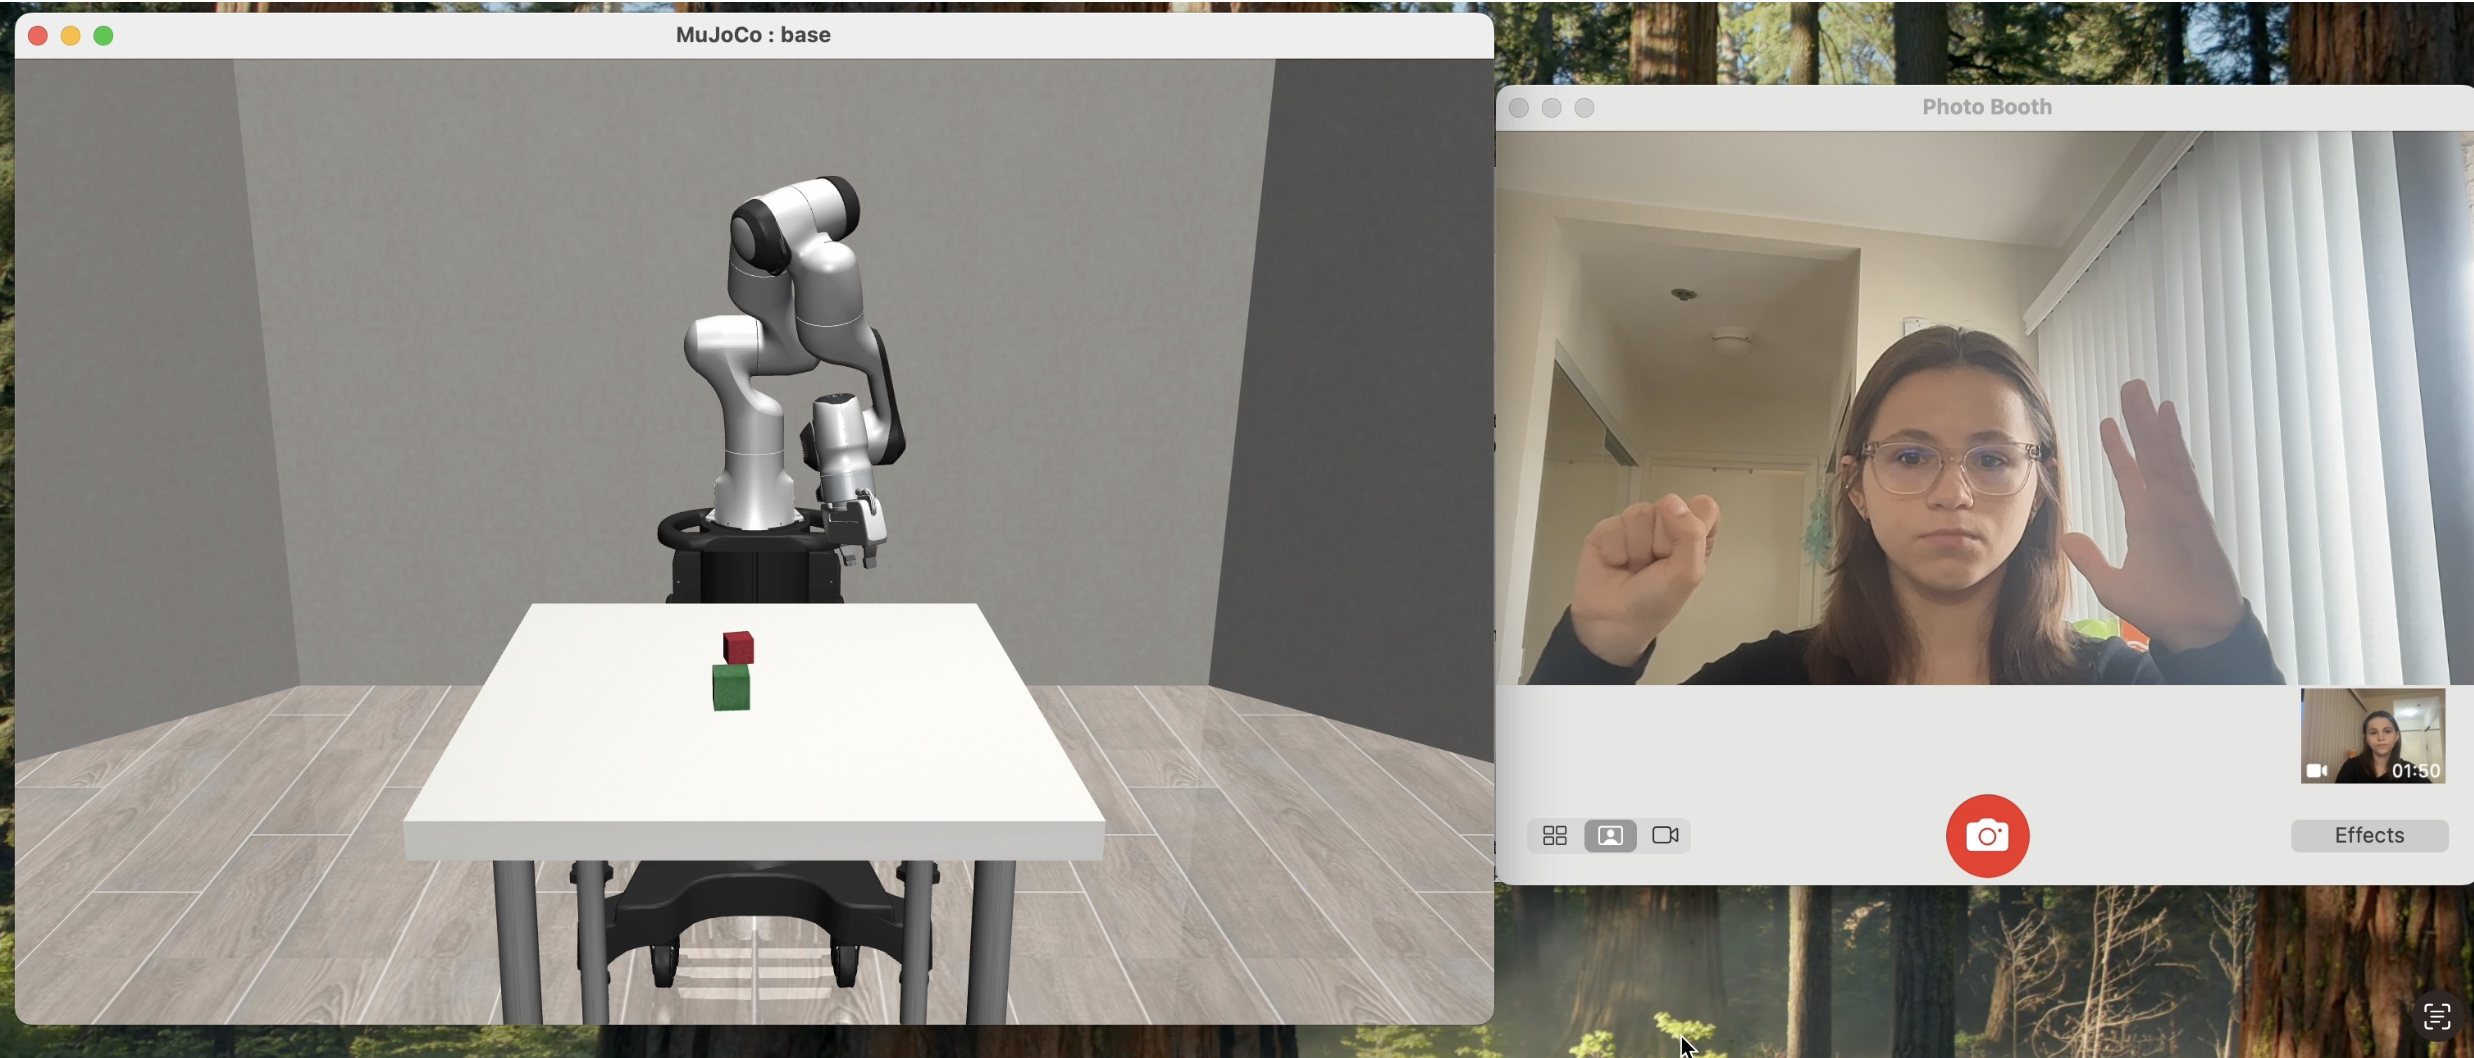
\includegraphics[width=0.7\textwidth]{../assets/fist-rotation.png}
  \caption{The robot follows the right hand's movement to rotate when the left hand is in a fist. }
  \label{fig:fist-rotation}
\end{figure}

%===============================================================================

\section{Evaluating Results}
\label{sec:result}
This project was successful overall, as the camera can track hand landmarks and
the robot end-effector can follow the user's hand movements in 3D. The robot
can follow the user's hand in real space and replicate it in the simulation in
3 dimensions. The robot can also follow the user's hand rotations to rotate its
end-effector, with some constraints due to both robot joint constraints and
constraints on the user's wrist. The user can pinch their thumb and forefinger
together to close the robot's gripper and release them to open the gripper (see
Figure \ref{fig:fist-rotation}). Isolating the rotation from translation
assisted us in completing tasks, as it is difficult for a user to concentrate
on rotation and movement at once when trying to manipulate in the 3D space. We
were able to use our hand controls to complete the Stack and Door tasks in
Robosuite as outlined in our proposal. We fulfilled our goal of allowing a user
to control a robot with just their laptop camera and no other physical
controllers.
\begin{figure}[H]
  \centering
  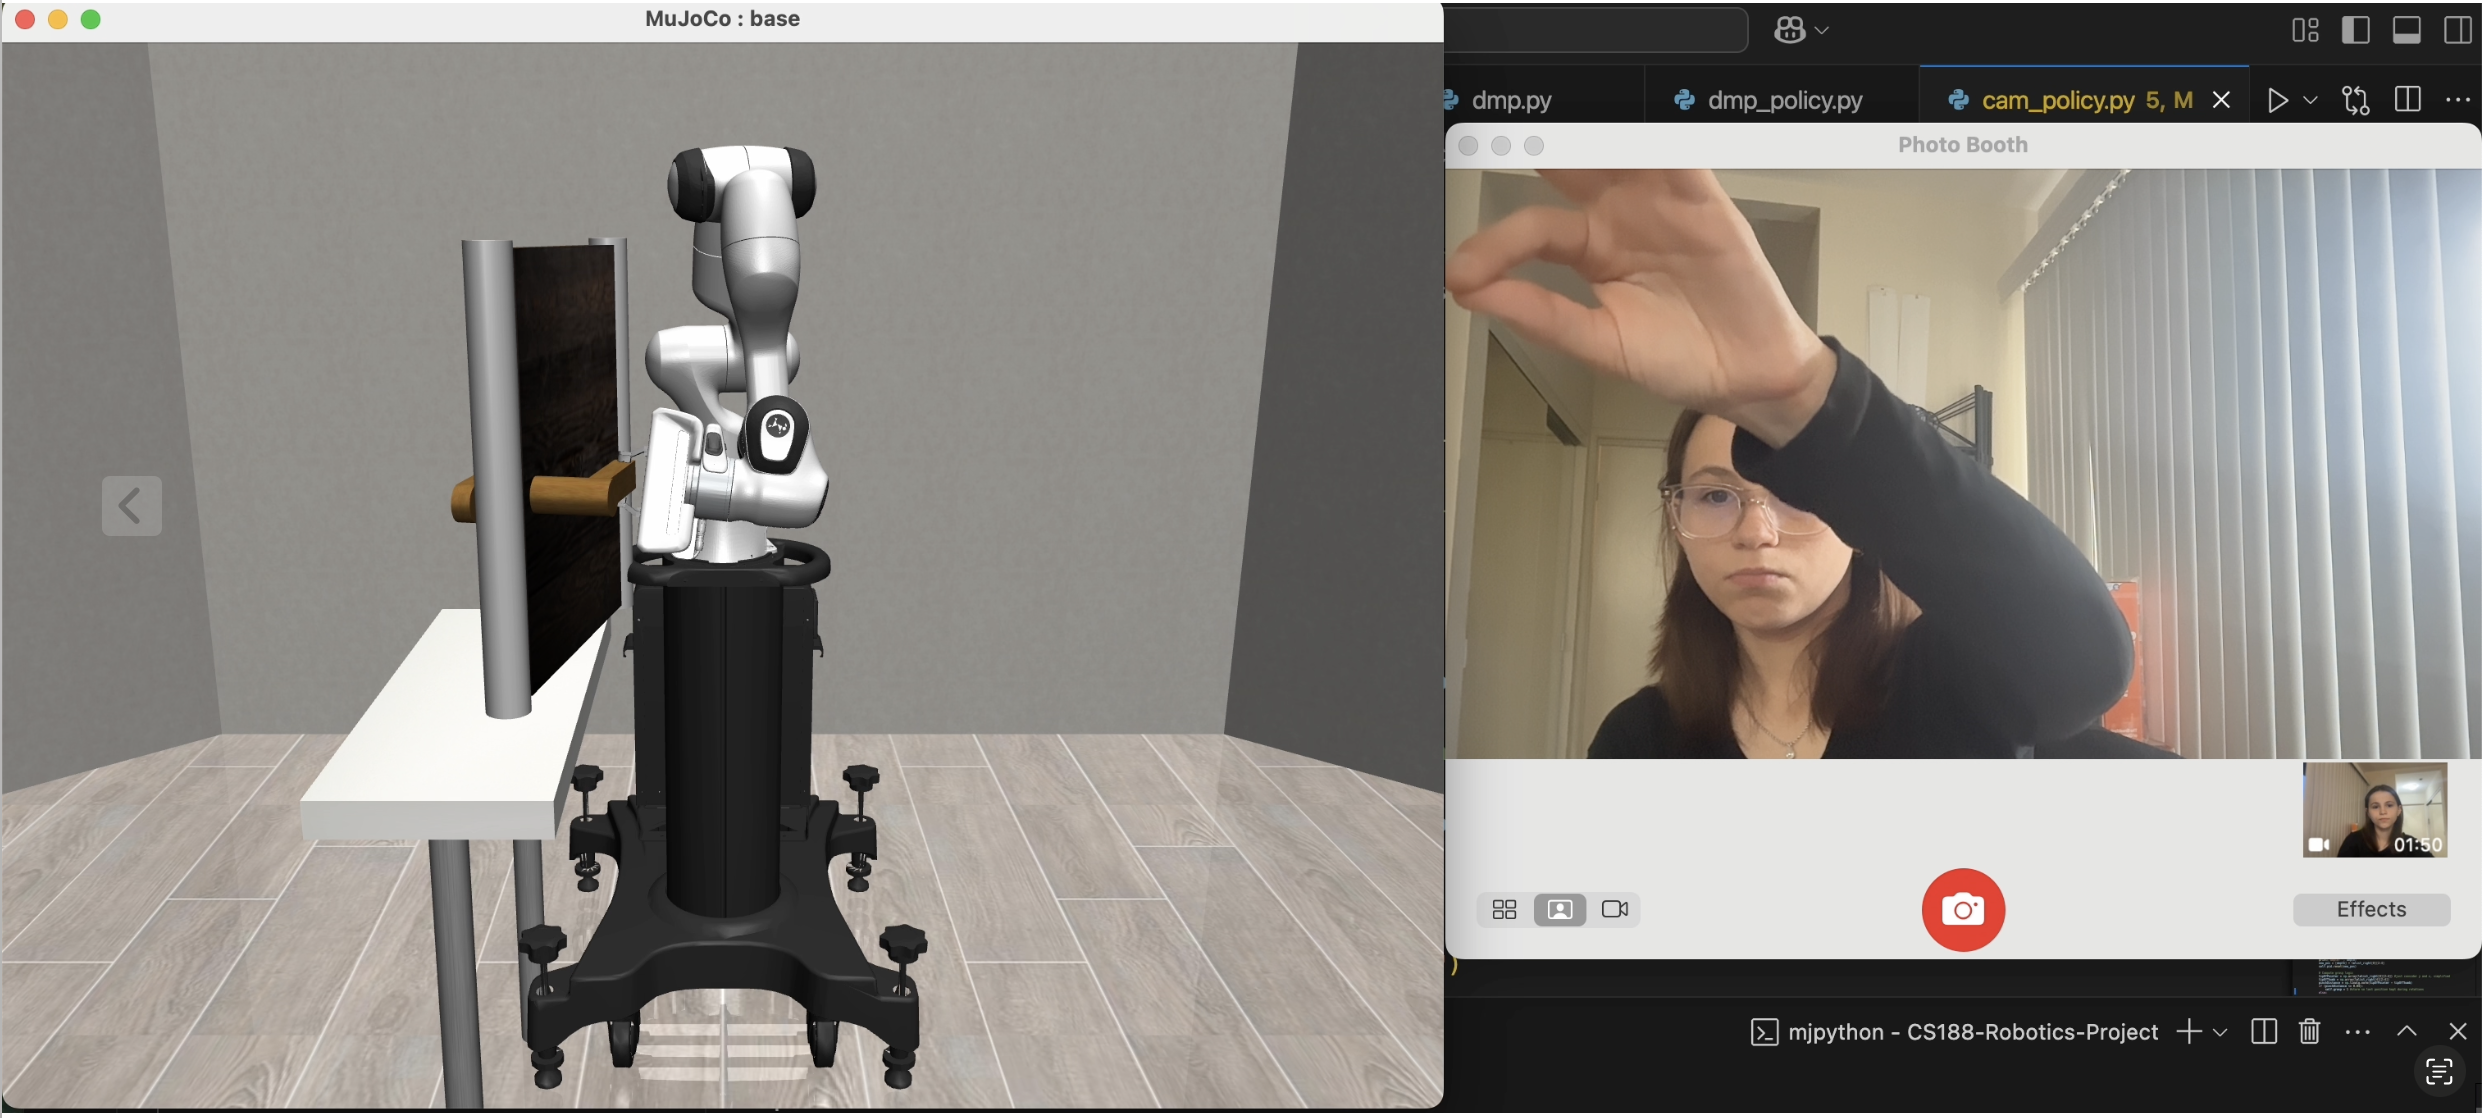
\includegraphics[width=0.7\textwidth]{../assets/gripper.png}
  \caption{The robot closes its gripper when the right hand has pointer and thumb pressed together.  }
  \label{fig:gripper}
\end{figure}
%===============================================================================

\section{Discussion \& Reflection}
\label{sec:conclusion}
\subsection{OpenCV on Mac}
We had some issues getting the camera to work and show up on Mac because Mac
requires GUI apps to run on the main thread, which OpenCV does not do
automatically. We decided to test camera tracking and robot testing separately,
so that the webcam tracking could be run with \texttt{python} and the robot
scripts could be run with \texttt{mjpython}. Since our test script includes the
webcam display by default, we added a script to check whether you were running
in \texttt{mjpython}; it will display the webcam view alongside the robot if
you run on a Windows machine and will just show the robot otherwise. This
allows our test script to run without errors on multiple platforms.

\subsection{Depth Tracking}
Before our final version of depth tracking, we also experimented with depth
tracking by calculating the area of the hand. The hand was approximated as a
triangle, and that area was calculated. Then the hand area could be stored in
the beginning and used to find a scalar for the current depth – if the hand
area is bigger than the start, it must be closer to the camera. Taking out the
depth coordinate and using the hand area helps estimations when the hand is
facing forward, but once the hand turns, the areas would no longer be very
accurate. This is because when the depth coordinate is excluded, as the hand
turns, the difference between 2 coordinates can decrease, making the hand area
smaller even if it hasn't moved away from the camera. Depth tracking is quite
difficult with one camera, and a future version of the project could use
another ML tool for estimating depth from one image. 

\subsection{Rotation Tracking}
We set up axes for the rotation using landmarks on the hand. However, this
became hard to visualize, so we attempted to add axes to the webcam view so you
can see what the hand axes were calculated as, but the axes struggled to
consistently stay correctly oriented as the hand rotated, so it was scrapped.
We had some issues with the robot being difficult to control once rotation is
incorporated due to joint constraints. When the robot is trying to follow both
a specific rotation and movement of your hand, it can end up trying to follow
impossible trajectories and get "stuck". It could also be difficult due to
real-life joint constraints on your hand. In certain wrist positions, a
movement that should be simple for the robot is difficult for the user to
actually perform, so some tasks become harder. Once we separated rotation and
translation, we updated the rotation to be based on a deviation from the "base
rotation" of the hand when the fist was first made by the left hand. This made
it easier to get the robot into certain rotations, as you could simply open the
fist, twist your right hand into a more comfortable position, and then re-close
the fist to continue the rotation.

\subsection{Fist Detection}
The fist detection has some limitations due to the camera not being able to see
the fingers once curled or when the hand is turned to the side. Because
MediaPipe hand detection decreases in poor lighting, the fist detection does as
well. We wanted to keep the detection fairly simple, so it is most accurate
when the fist faces forward and the hand is not forcefully tightened. Having
the ability to drop the left hand when not doing rotation is very useful, so
your left arm doesn't get tired during manipulation. It was also very useful to
be able to set a specific rotation and then apply translations.

\subsection{Takeaways}Overall, controlling a robot via hand movements can be
quite finicky, especially as you are trying to interpret depth onscreen and
figure out how to move your own hand to a correct position. It can require a
good deal of hand-eye coordination and can get tiring over time. The hand
tracking could be more useful for fine-motor tasks using a robot with
controllable fingers, rather than for broad movements and basic gripping like
the Panda robot. In the future, it would be interesting to program a robot to
do tasks associated with general hand movements; for example, rather than
directly following the hand, the robot could use dynamic movement primitives to
determine a good trajectory to move in the direction you indicated. 


%===============================================================================
\section{Team Contribution Division}
%===============================================================================
\subsection*{Alexander}

Xander set up the initial hand tracking and camera policy. He implemented depth
tracking computation with added smoothing to reduce jittery movements.
Additionally, he developed the rotation tracking computation and added
landmarks to hand positions to assist with the rotation calculations.

\subsection*{Brenna}

Brenna worked on debugging the initial setup and handled coordinate system
conversions from MediaPipe to Robosuite. She implemented 2D translational
movement for the robot based on hand tracking and began work on 3D movement
with depth calculations. She added detecting whether the user is running with
\texttt{python} or \texttt{mjpython} to toggle showing the webcam view. She
also added fist detection to isolate translation and rotation controls. 

\subsection*{Clayton}

Clayton added better error handling for edge cases and contributed to general
research on the project. He did general testing and tuning to try to smooth out
the robot movements relative to hand movements. He ensured the
project worked well cross-platform and debugged depencency issues. He also designed
and deployed the website for the project.

\clearpage
% The acknowledgments are automatically included only in the final and preprint versions of the paper.
\acknowledgments{Thank you to Yuchen Cui, Seth Zhao, and Raayan Dhar for all their help with learning robot planning and control in Robosuite!}

%===============================================================================

% no \bibliographystyle is required, since the corl style is automatically used.
\raggedright
\bibliography{report}  % .bib

\end{document}
